Free-Riders operate by pretending to act as a normal client that is contributing to a model, all while actually contributing nothing.
To successfully achieve this and convince the central server, several clever tactics need to be undertaken to hide as best as possible.
This chapter will be investigating their effectiveness and seeing how well robust aggregators are able to handle them.
The main points of interest will be accuracy and which clients get blocked.
\\ \\
All experiments done have been run on all the previous aggregators. 
In terms of StD and mean tests (as described later), there does not appear to be much difference in distinction.
So FedAvg shall be used for these types of graphs in this section unless otherwise stated.

\section{Main Measure of Defence}
The best way to detect the free-riders from attacks is through the mean and StD of the parameters gradient weights.
Standard clients tend to show a general noisy shape that has an initial increase and then slowly decreases to flat as the model converges [\ref{fig:std_basic}].
\begin{figure}[htbp]
	\centering
    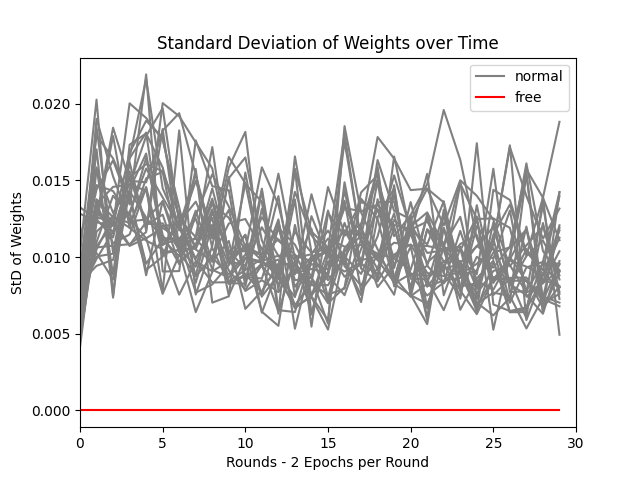
\includegraphics[scale=0.5]{free_riders/graphs/1_free.png}
	\caption{StD Curve for Most Clients Compared to Free-Rider}
	\label{fig:std_basic}
\end{figure}

As you can see, free-riders will have to try and match this general shape in order to stay hidden. 
However, it may be that the central server doesn't find itself in a position where it cares unduly.
Looking at the case where there are 5 free-riders in a basic attack [\ref{fig:5free}], the accuracy tends to be really good all-round with the slight exception of FedMGDA++.
If the main concern of the central server is simply the accuracy at the end of the model, then ultimately it may not be considered an issue.
However, if there is intellectual property or monetary value at stake, free-riders might not be acceptable.


\section{Noise Addition}
For the central server, if all it received was the same model that it sent out, it would be easy to tell which clients are free-riders. 
To counteract this check, the free-riders can simply add some noise to the model so that they can remain more hidden.
This does allow for some more basic blending in but does not quite achieve the same necessary shape. 
However, it is able to demonstrate an ability to give an appearance of remaining hidden [\ref{fig:std_noisy}] through similar visual noise characteristics.
\begin{figure}[htbp]
	\centering
    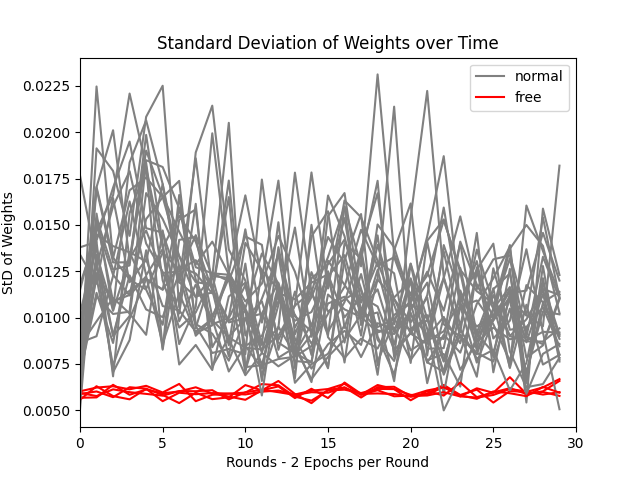
\includegraphics[scale=0.5]{free_riders/graphs/noisy5.png}
	\caption{StD Curve for 5 Noisy Free Riders}
	\label{fig:std_noisy}
\end{figure}

Initially, it might look like there is a blatant distinction between the 2 sets of clients.
However, the noise parameters can be finely tuned such that they can match the amplitude and displacement as is present with the benign clients.
Therefore, the clients can much more seamlessly blend in.
\\ \\
One issue that remains, is that the tuning from the free-riders is somewhat a tricky matter.
From an outside perspective with full control of the system, it can easily be decided what the noise parameters should be.
However, from a free-rider with information only about the global model and itself, it cannot know for sure what the optimal parameters are.
This can be subsidised by investigating the difference in the models and to try and calculate ideal noise patterns from that, but it still lacks accuracy and can ultimately be detected through analysis or through DAGMM energy.

\section{Delta-Weights}
This is where the delta-weight attack comes in.
The idea follows on from the previous section on estimating the noise parameter values whereby you take the delta between the current global model and the previous one.
The difference is then taken and is set to be the free-rider's model gradient weights.

\subsection{Standard Attack}

This has the useful side-effect of having the StD and the mean of the gradient weights to more closely emulate that of a standard client as shown in [\ref{fig:std_delta}].
\begin{figure}[htbp]
	\centering
    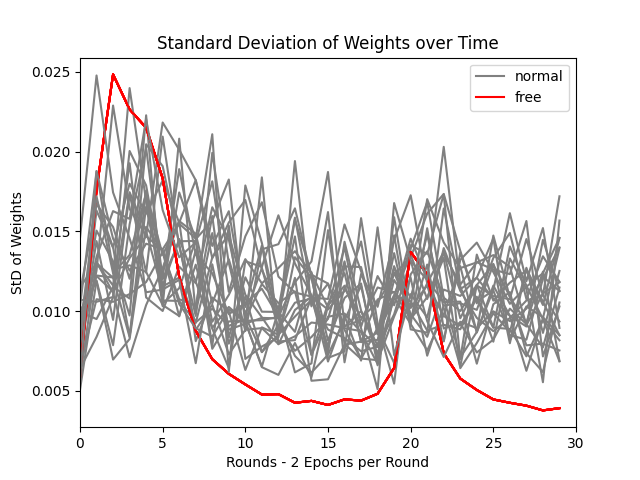
\includegraphics[scale=0.5]{free_riders/graphs/delta8.png}
	\caption{StD Curve for 8 Delta-Attack Free Riders}
	\label{fig:std_delta}
\end{figure}

Now, it's obviously not a perfect solution but it does show the more characteristic increase at the beginning along with the second peak later on that more closely resembles the other clients.
Again, it is not a ultra-finely tuned system but definitely approaches a solution that much more closely resembles a correct one.
\\ \\ 
One basic detection method would be to just check if there are any clients with identical StD characteristics but obviously this attack would benefit from some noise and scaling in places.
This is important to note as ultimately there are an endless amount of possibilities of fine-tuning a free-rider could do to any attack vector and so getting bogged down in the nitty-gritty doesn't contribute much.


\subsection{Privacy Amplification with User Sampling}
When adding privacy amplification, it is important to know if there are points at which the convergence will break down.
This is because it may be that there are just simply too few clients in each aggregation step to do so properly.
Now currently, IID data is being used and so the likelihood of this is not too high, but it is something to at least test and consider.
For the experiments, the value at which the uniform sampling will be cutoff is the p-value and this is what will be altered.
\\ \\
As assumed, the performance degradation is practically none for IID data [\ref{fig:p_test}] with only MKRUM showing some performance loss with very small p-values (0.05 - 0.01).
This only happens for higher number of epochs per round. 
When it is reduced from 10 to 2 (our previously calculated ideal), we see that MKRUM fails much more spectacularly [\ref{fig:p_test_2}] on the lower p-values.
As the clients are sampled uniformly and randomly, it is enough to conclude that the thresholding value does not provide too much of an issue to the performance of the model.
It should be noted that with the addition of malicious/faulty/free-riding clients, the effects of larger amounts of these clients may become exaggerated when the p-value is too low.


\subsection{Privacy Amplified Attack}
With the most advanced attack being based on the difference of 2 models, it stands to assume that you ideally do not want the clients to have the global model at all to help reduce this attack.
This might not be sensible as the clients could need the global model to converge properly.
So instead, if we were to then reduce the amount of time the clients got hold of the model, then their attack would be less deceptive and become clearer to the outside viewer.
With the help of privacy amplification, we can do just that.
For testing, I used a p-value of 0.3 as a good balance between wanting to maintain accuracy but also wanting to minimise frequency of contribution.
\\ \\
You can see the effects in [\ref{fig:std_priv}] quite clearly and the free-riders are much more noticeable.
\begin{figure}[htbp]
	\centering
    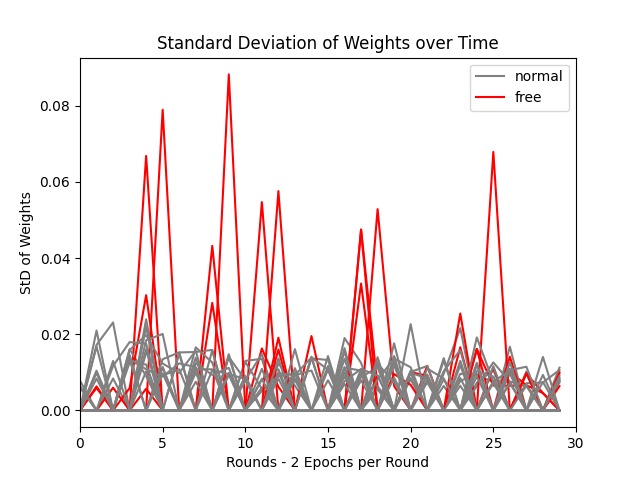
\includegraphics[scale=0.5]{free_riders/graphs/priv5.png}
	\caption{StD Curve for 5 Free-Riders using a Delta-Attack while under Privacy Amplification}
	\label{fig:std_priv}
\end{figure}

The graph shows a lot of data at zero as well and that's just because the gradient weights will be non-existent if they haven't been trained.


\section{Robust Aggregation}
The method by which typical robust aggregators go about aggregating is through identifying and not including outliers (or weighting them low) in the process.
However, by their very nature, free-riders are not outliers in the sense that their parameters are very benign if anything.
They are the essentially the most medium clients from the previous round. 
It is unlikely they would be detected at all by the robust aggregators.

\subsection{Performance}
There was also the matter of performance as having degraded model performance with aggregators trying to do fancy things is really not ideal.
On the low end, performance was not an issue an across the board [\ref{fig:no_dmg}] and only with the addition of privacy amplification did MKRUM suffer [\ref{fig:mkrum_suf}] even with very few free-riding clients.
\\ \\
In general, the performance of the models slowly decreased as more free-riders were added.
FedMGDA++ and MKRUM were more badly affected but it was very much a gentle decrease.
The more interesting point to note was the transition over the halfway point [\ref{fig:comed_broken}] where it went from 14 to 16 malicious free-riders.
This is noteworthy due to it again highlighting COMED's weakness around this point as an aggregator and how it so quickly falls down.
Especially as the other aggregators then proceed to essentially not change much more than normal and are capable of aggregating at a rate such that the decline in accuracy is fairly constant.
\\ \\
The reason the other aggregators don't fall short as badly, is because the free-riders act more as an LR softener.
Essentially, they slow down the rate at which the model converges as you are just adding a bunch of dampening parameters, that are the previous model, to the next global model.
This is why you mainly just see the curves for things like FedAvg, AFA and MKRUM just be at a shallower angle as opposed to having the final position be too much higher.
\begin{figure}[htbp]
	\centering
    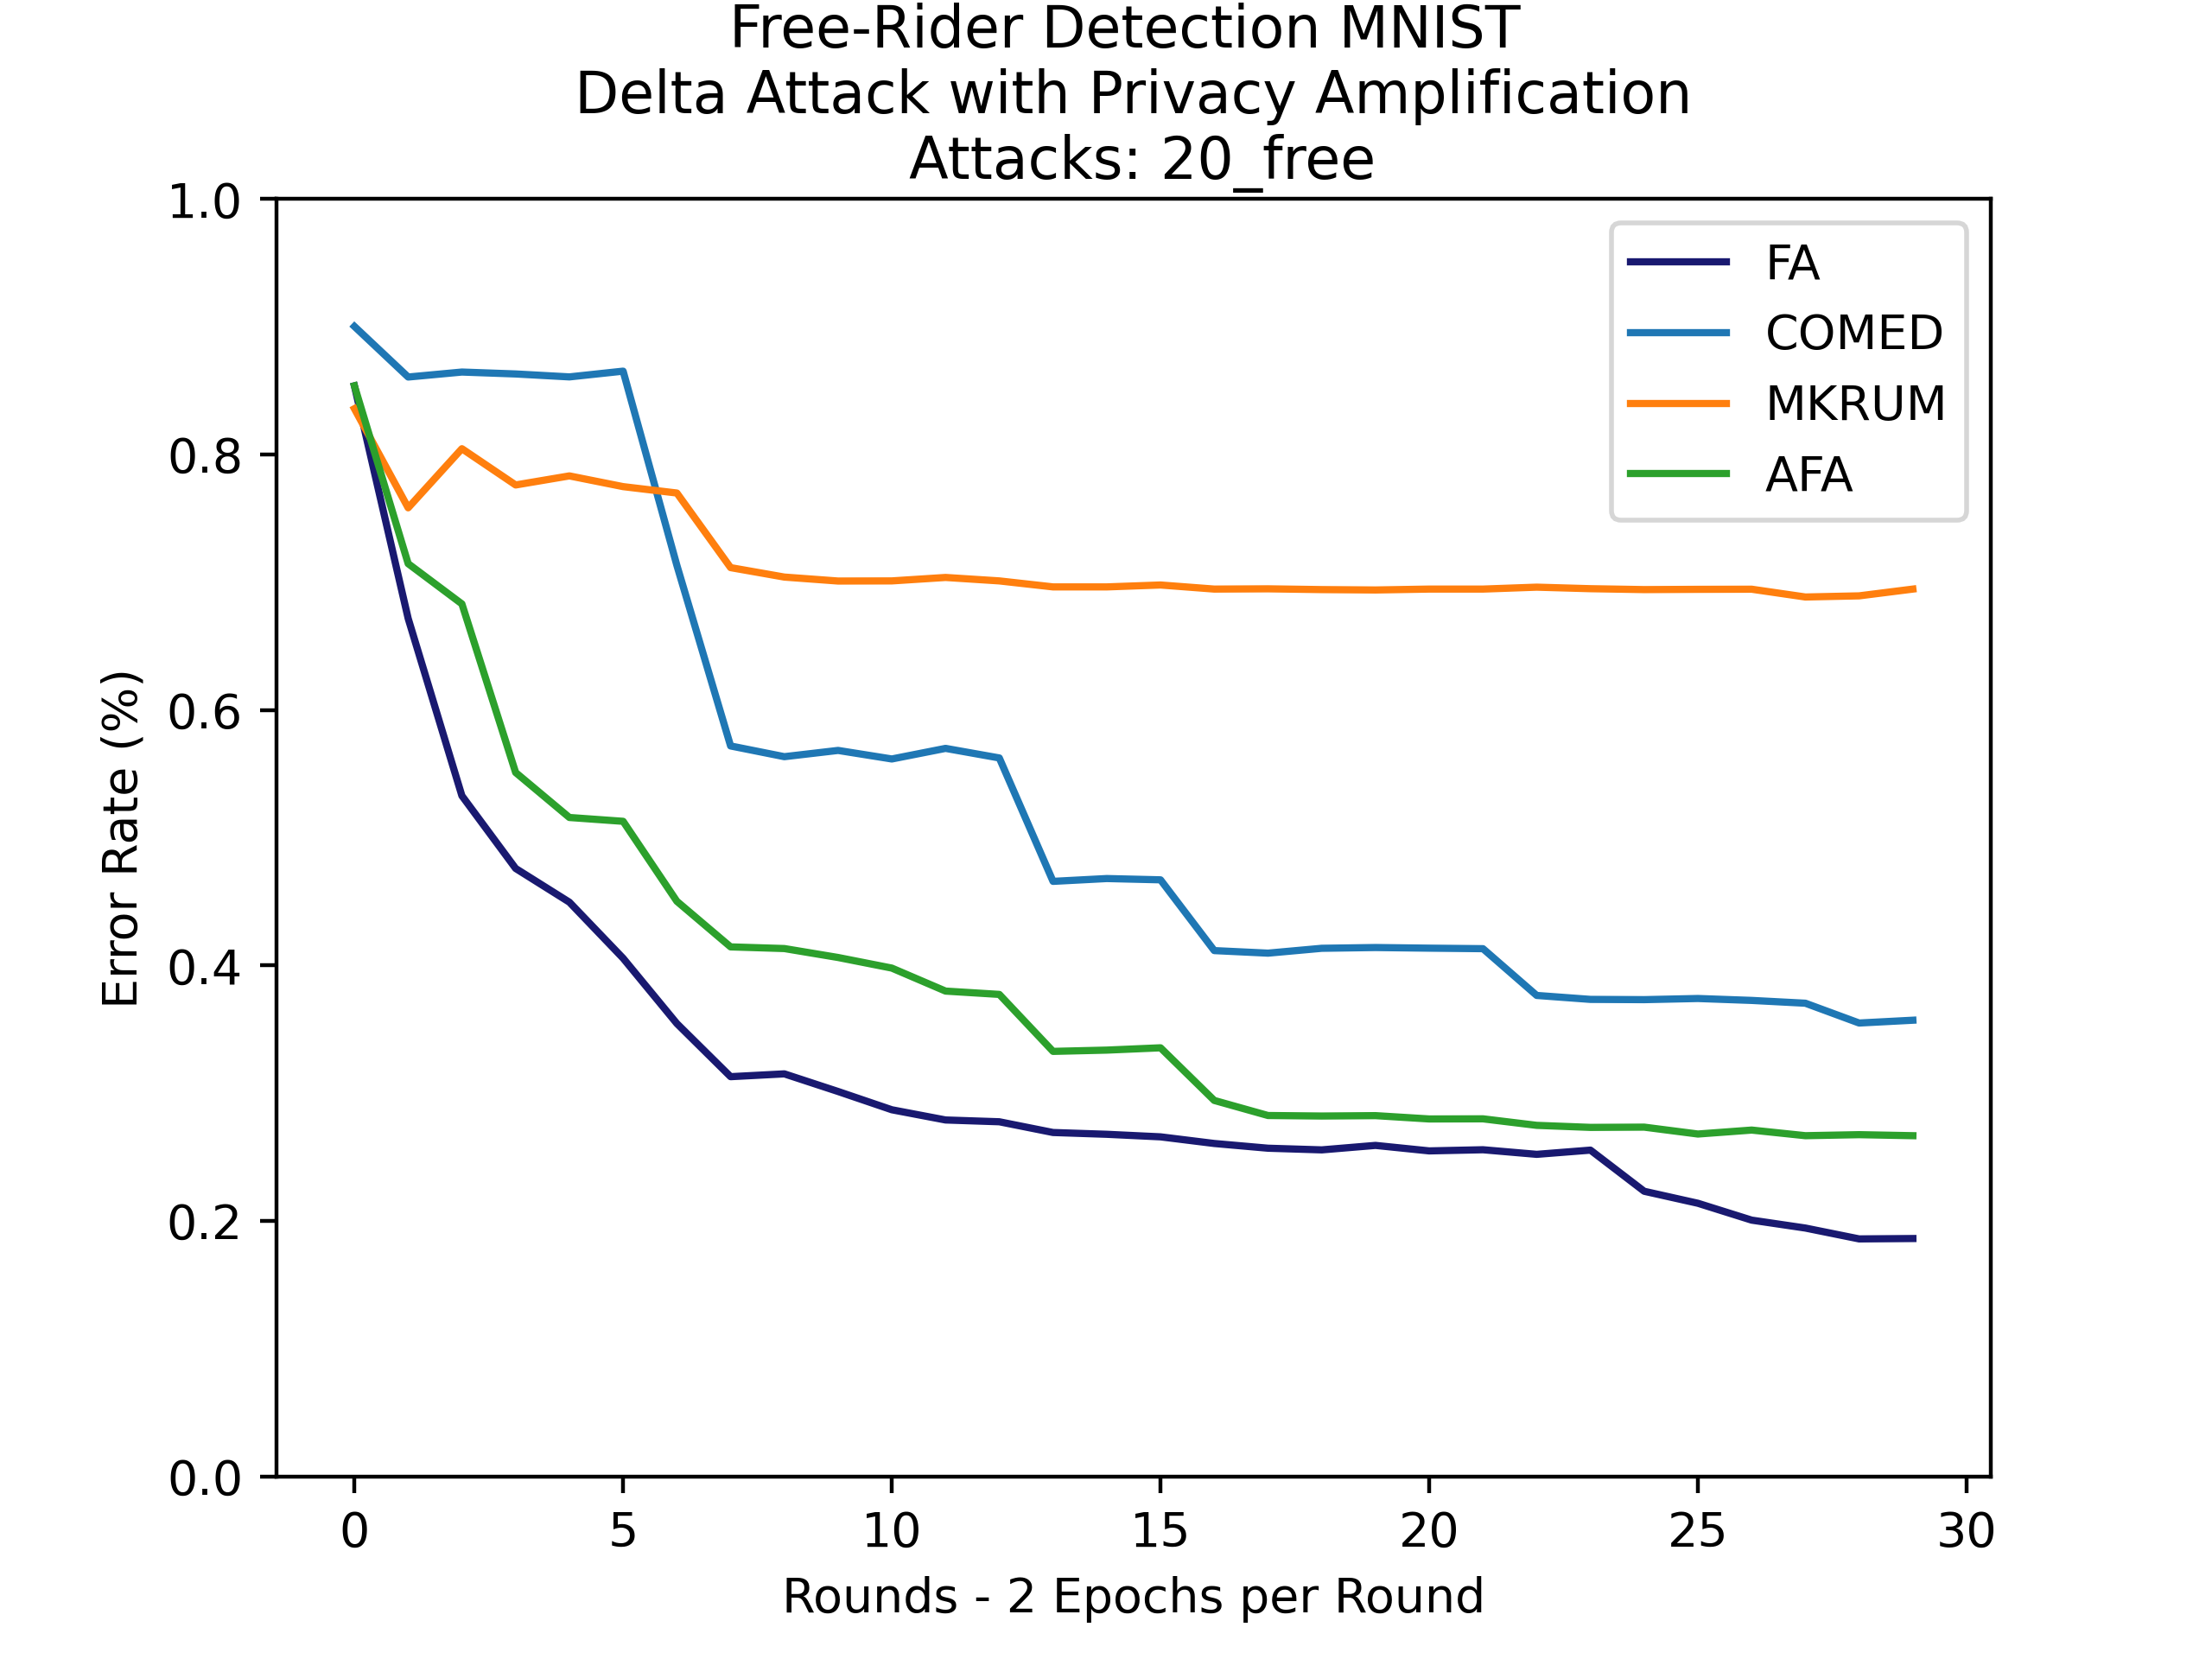
\includegraphics[scale=0.5]{free_riders/graphs/priv20.png}
	\caption{Error Rate of 20 Free-Riders with Delta-Weight Attacks under Privacy Amplification}
	\label{fig:priv20}
\end{figure}

The one exception to this is then the privacy amplification defence, where all of the aggregators are seen to be struggling much more in comparison [\ref{fig:priv20}].
What's fascinating is seeing the sudden drops that occur with COMED, which shows that when the sampling has chosen a set of clients that contains more than 50\% benign.
This leads to a conclusion that might seem odd at first.
If you were to be prioritising the accuracy of the model, then you'd actually not want to employ the privacy amplification defence as it does more damage than just letting the free-riders be.

\subsection{Blocking Issues}
One thing that stood out to me initially was the very poor performance from FedMGDA++ and how it noticeably became to worst affected as the number of free-riders increased.
It ended up being quite a simple issue, the aggregator was pretty much just identifying the benign clients to be the outliers!
This was happening as early on as with only 2 free-riders and 10 benign clients were getting blocked!
\\ \\
The main factor which caused the decrease in the accuracy was simply that with more free-riders, FedMGDA++ thought itself to be getting more certain as to which clients were malicious when in fact it was doing the complete opposite.
This caused the benign clients to be getting blocked earlier and earlier and that's what causes the flat-lining that you see in experiments such as [\ref{fig:flat_line}].
This carries onto about the 15\textsuperscript{th} round, where from then on out, all of the benign clients are getting blocked and so no learning can take place.
This happens to AFA too at higher free-rider counts but to a much lesser extent and AFA never blocks more than 5 benign clients, lending it to still be able to learn at a decent-ish rate.


\section{Conclusion}
Overall, free-riders provide an interesting problem in the field of federated learning.
On the one hand, they do very minimal damage and cannot be simply detected and blocked using traditional robust aggregation methods.
On the other hand, they can be capable of masking themselves with fake informational noise to great extents and are ultimately providing fake information to the global model.
\\ \\
It poses a peculiar threat and yet through evaluation of the performance, seems to show no characteristics of being one.
Now, robust aggregators weren't built for this purpose and that is precisely why other methods for detection have been covered.
Ultimately, the global model would benefit more without them and the clients behind the free-riders are getting this model for free and so it really comes down to whether or not either of these things matter much to the specific situation.
